\documentclass[letterpaper,12pt]{article}
\usepackage{graphicx}
\usepackage{subcaption}
\usepackage[english]{babel}
\usepackage{fancyhdr}

\graphicspath {{figures/}}

\setlength{\headheight}{15pt}

\pagestyle{fancy}
\fancyhf{}
\lhead{\textbf{Version:} 1.1  \textbf{Revision:} 11/02/17}
\rhead{\thepage}
\lfoot{Cole Kampa}
\rfoot{\textit{Mu2e: University of Minnesota}}

\renewcommand{\footrulewidth}{1pt}


\begin{document}
\begin{titlepage}
	\centering
	\includegraphics[width=0.5\textwidth]{mu2e_logo_oval.png}\par\vspace{2cm}
	{\scshape\LARGE Electronics Assembly for CO$_2$ Leak Testing: Co$_2$ Box\par}
	\vspace{3cm}
	{\Large Cole Kampa\par}
	\vspace{3cm}
	{\large University of Minnesota\par}
 	\vspace{.5cm}
	{\large November 2, 2017\par}
	% Bottom of the page
	\vfill
	{kampa041@umn.edu\par}
\end{titlepage}

\clearpage
\setcounter{page}{2}


\section{Goal}
We aim to manufacture 50 CO$_2$ leak testing units that will be used to verify that straws used in the tracker do not leak above a certain limit. There will be two stations of 25 leak chambers each. At each station, 5 Arduino units are configured to collect data from 5 CO$_2$ sensors each. The sensors are housed with a brushless DC fan in a die cast aluminum box fit with an airtight 4 pronged connection that gets connected to the Arduino unit. The lid of this unit (referenced as CO$_2$ box) is fit to the copper tube leak chambers. This report focuses on assembling the CO$_2$ boxes. We strive to do this in a safe, efficient, and reproducible manner.



\section{Equipment}
	\begin{itemize}
		\item Tooling
    		\begin{itemize}
			\item Soldering iron
			\item Hot glue gun (standard)
			\item Helping hands stand with two movable arms and alligator clips
			\item Yellow wire stripper
			\item Razor blade
			\item Needle-nose pliers
			\item Flathead screwdriver
			\item Ruler
			\item Lighter
			\item Cotton swab
		\end{itemize}
		\item Materials
    		\begin{itemize}
			\item Die cast aluminum enclosure (NEMA 4 AN-1300-G)
			\item EE893 (or EE891) CO$_2$ sensor (Note: figures in this document use the EE891 model)
			\item Brushless DC Fan Model OD2510-05HB (5V, 0.14A)							
			\item Custom G-10 base
			\item Amphenol Industrial PT02E-8-4P (referred to as 4-pin connector)
			\item Sealing gasket for \#8 wall receptacle (for 4-pin connector)
			\item 30 AWG flexible silicone coated wire (red, green, yellow, black) (2.5" each)
			\item Narrow shrink tube (red, green, yellow, black) (3/4" each)
			\item Right-angled header pins (0.1" separation) (4 broken off as one unit)
			\item Solder
			\item RTV (Note: Corrosive, do not apply to any of the electronic components)
			\item 1/2" 2-56 pan head slotted machine screws (3)
			\item 2-56 3/16" steel hex nuts (9)
			\item 1/4" 4-40 pan head slotted machine screws (4)			
		\end{itemize}
	\end{itemize}



\section{Risks and Dangers}
	\begin{itemize}
		\item RTV: \\
		\textnormal{Make sure to work in a well ventilated area, as RTV produces acetic acid vapor while curing. This can cause eye irritation. Avoid contact with skin. Thoroughly rinse if any RTV contacts skin.}
		\item Soldering: \\
		\textnormal{The solder contains lead, a neurotoxin. As such, avoid inhaling the fumes created when solder is heated. The soldering iron is hot. Work in a cleared area to avoid burns.}
	\end{itemize}

\newpage

\section{Diagram} \label{diagram}
%\subsection{Sensor Box}
	\begin{figure} [!htb]
		\centering
		\includegraphics[width=1\textwidth]{diagram_1.png}
		\caption{Diagram of CO$_2$ box circuitry.}
		\label{fig:diagram}
	\end{figure}

%\subsection{Overall System}

%\includegraphics[width=\textwidth]{}



\section{Methods}
\subsection{Preparation}
	\begin{enumerate}
		\item General: \\
		\textnormal{The aluminum box should already have 5 holes drilled on one of the long edges. The large hole is for the 4-pin connector to fit through while the smaller holes are threaded for the 4-40 machine screws to hold the 4-pin connector in place. If the sticker is still on the inside of the box, remove it. The CO$_2$ sensor should be tested using the Arduino debug code with the test header/4-pin connector.}		
		\begin{figure}
			\centering
			\begin{subfigure}{.45\textwidth}
  				\centering
				\includegraphics[width=\linewidth]{4pin_pliers.png}
				\caption{Positioning of pliers.}
				\label{fig:4pin_pliers}
			\end{subfigure}
			\begin{subfigure}{.45\textwidth}
				\centering
				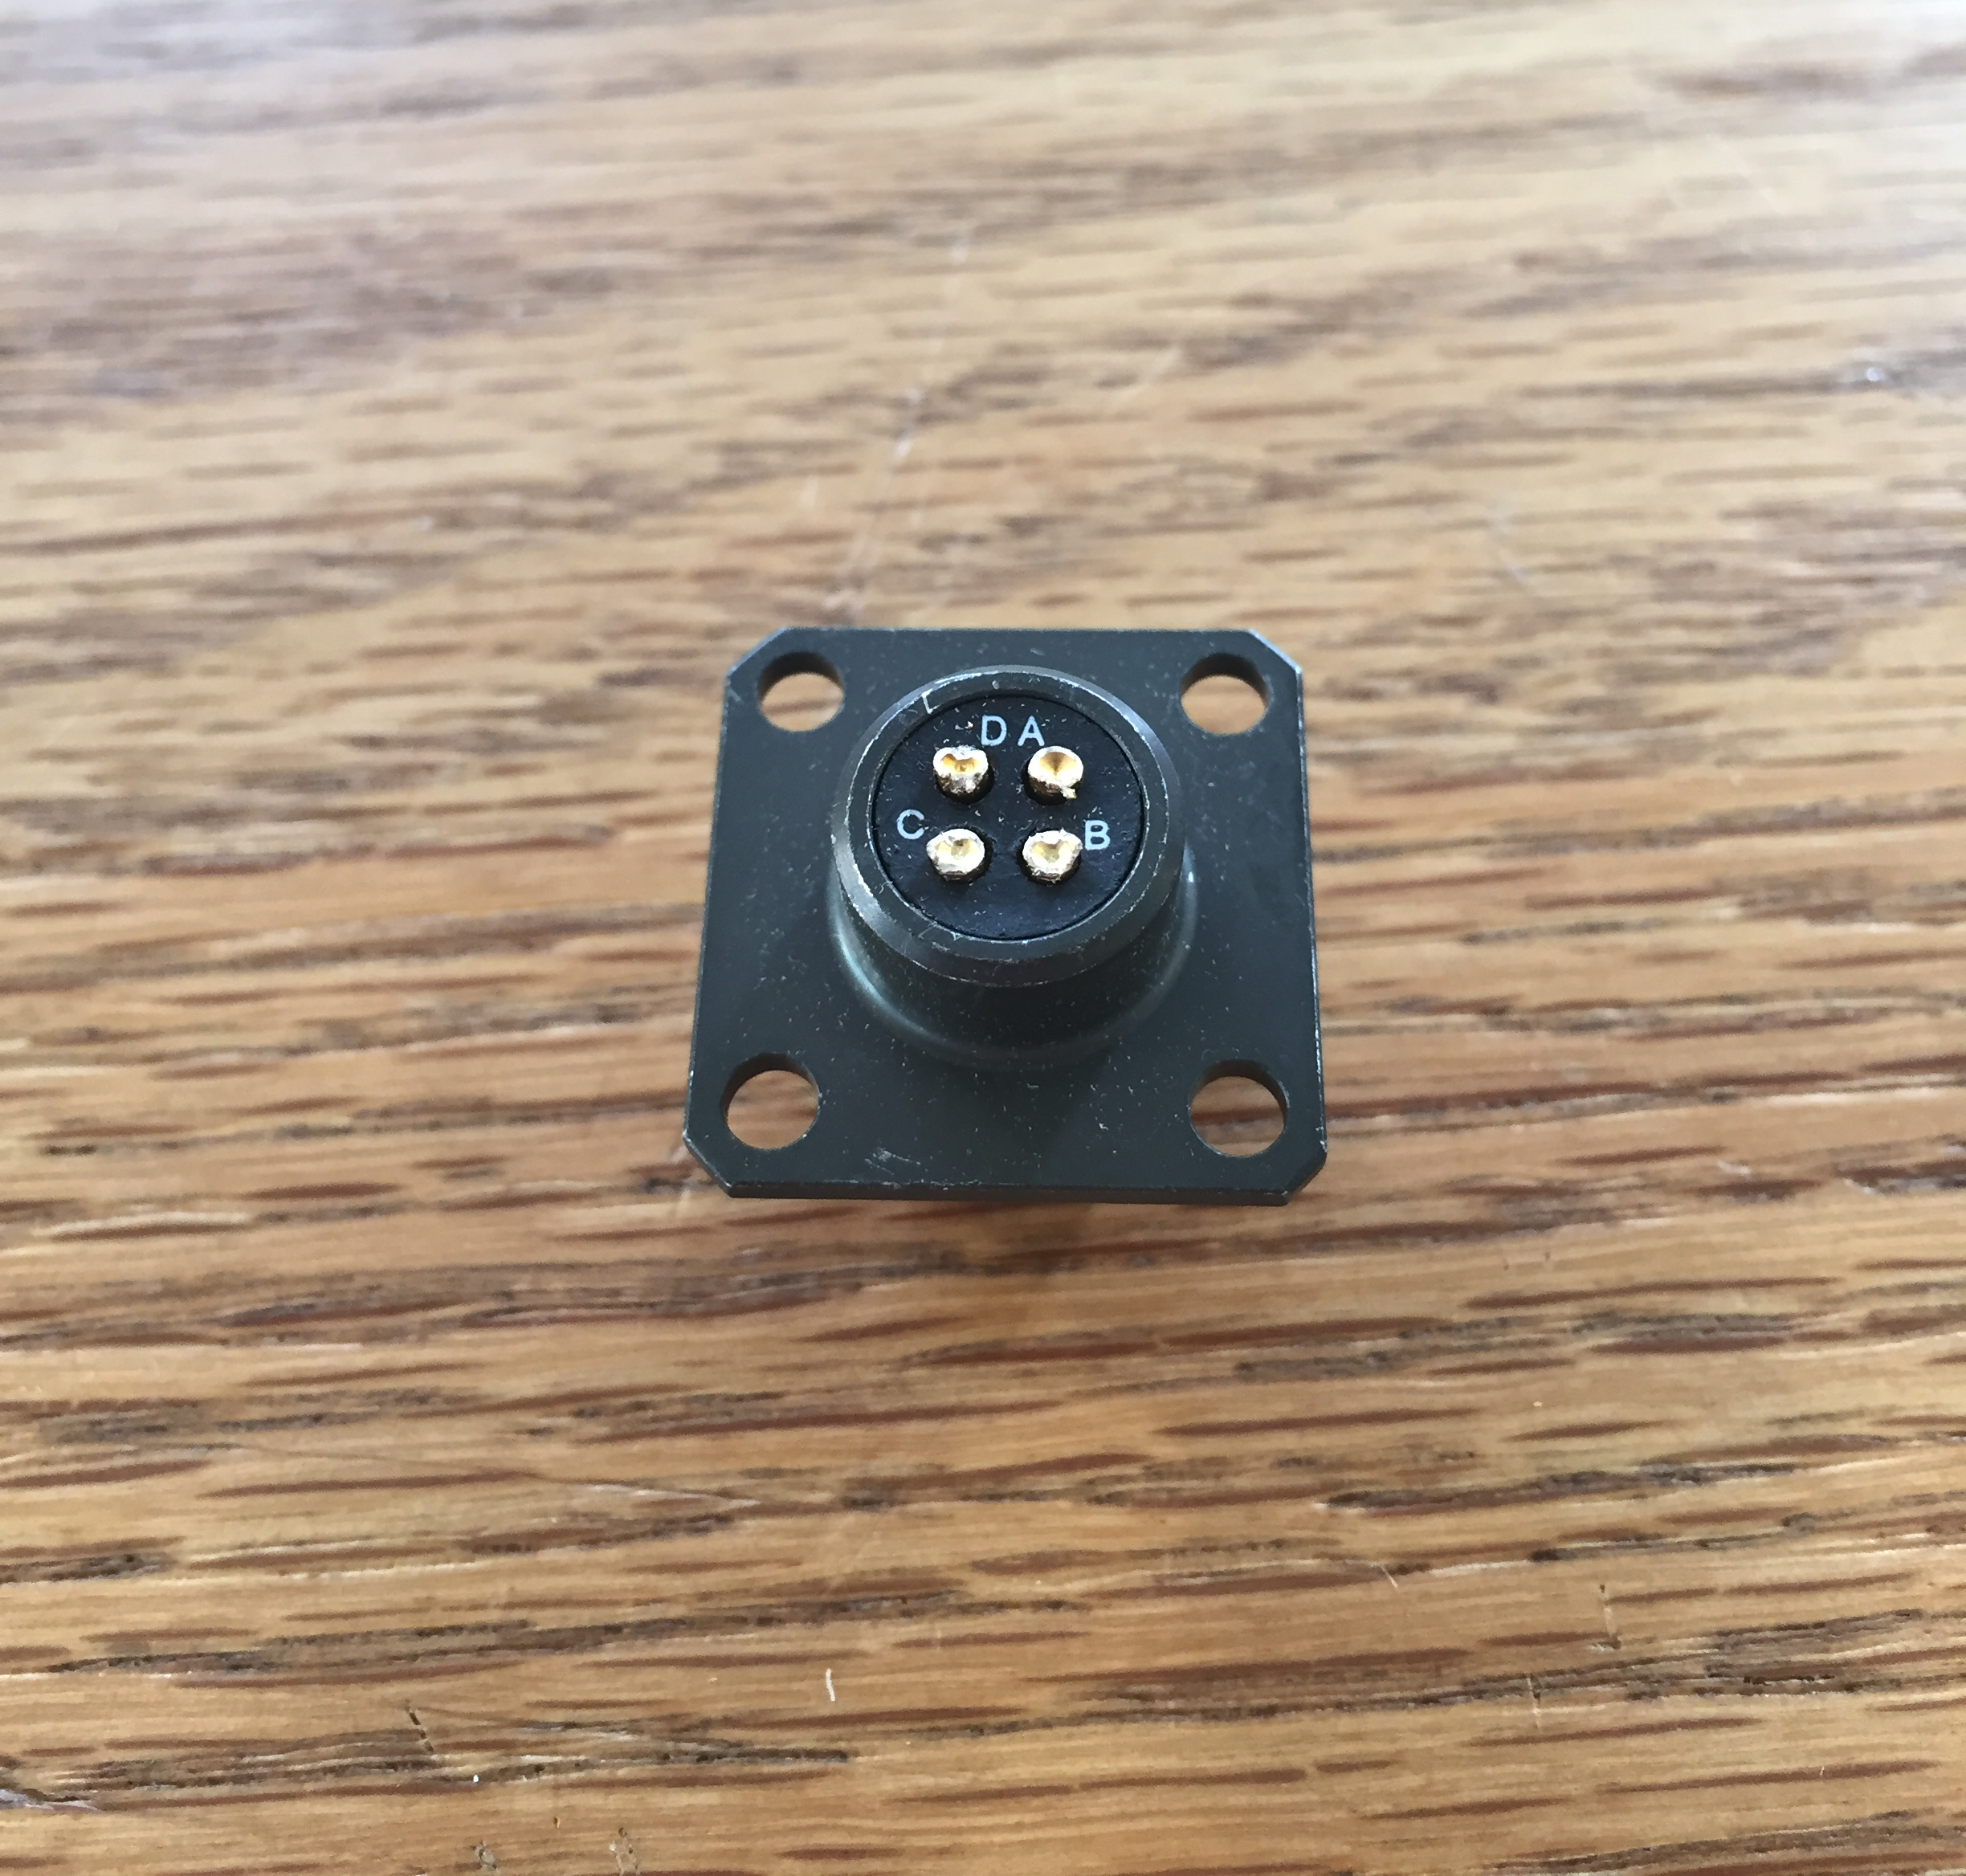
\includegraphics[width=\linewidth]{4pin_after.png}
				\caption{4-pin after breaking wells off.}
				\label{fig:4pin_after}
			\end{subfigure}
			\caption{Breaking off the 4-pin connector metal wells to fit in enclosure.}
			\label{fig:4pin}
		\end{figure}
		\item 4-Pin Connector: \\
		\textnormal{With the cheaper model of the 4-pin connector that we are using, the base protrudes too far into the aluminum enclosure. The metal wells on the back must be shortened down to the base. This is done easily by using a pliers as shown in figure~\ref{fig:4pin_pliers}. While squeezing the pliers, slowly twist each metal well off. The result should resemble figure~\ref{fig:4pin_after}.}
		\item Wiring \& Soldering:
		\begin{itemize}
			\item Cut a 2.5" length of each of the four colors of wire used in the CO$_2$ box. Strip 1/4" of insulation from each end using the smallest position of the yellow wire stripper. If necessary, carefully remove excess insulation using a razor blade.
			\item  Following the wiring scheme outlined in section~\ref{diagram}, first solder each wire to the adjusted 4-pin connector. To do this, hold a wire vertically in place above the 4-pin connector with the helping hands so that the wire sits in the remainder of the well. Ensure the soldering iron touches the wire and the well to ensure a solid solder joint.
			\item Cut two 3/8" lengths of shrink tube in each of the four colors. Slide each pair of tubes onto the corresponding colored wire so that it rests directly above the 4-pin connector.
			\begin{figure} [h]
				\centering
				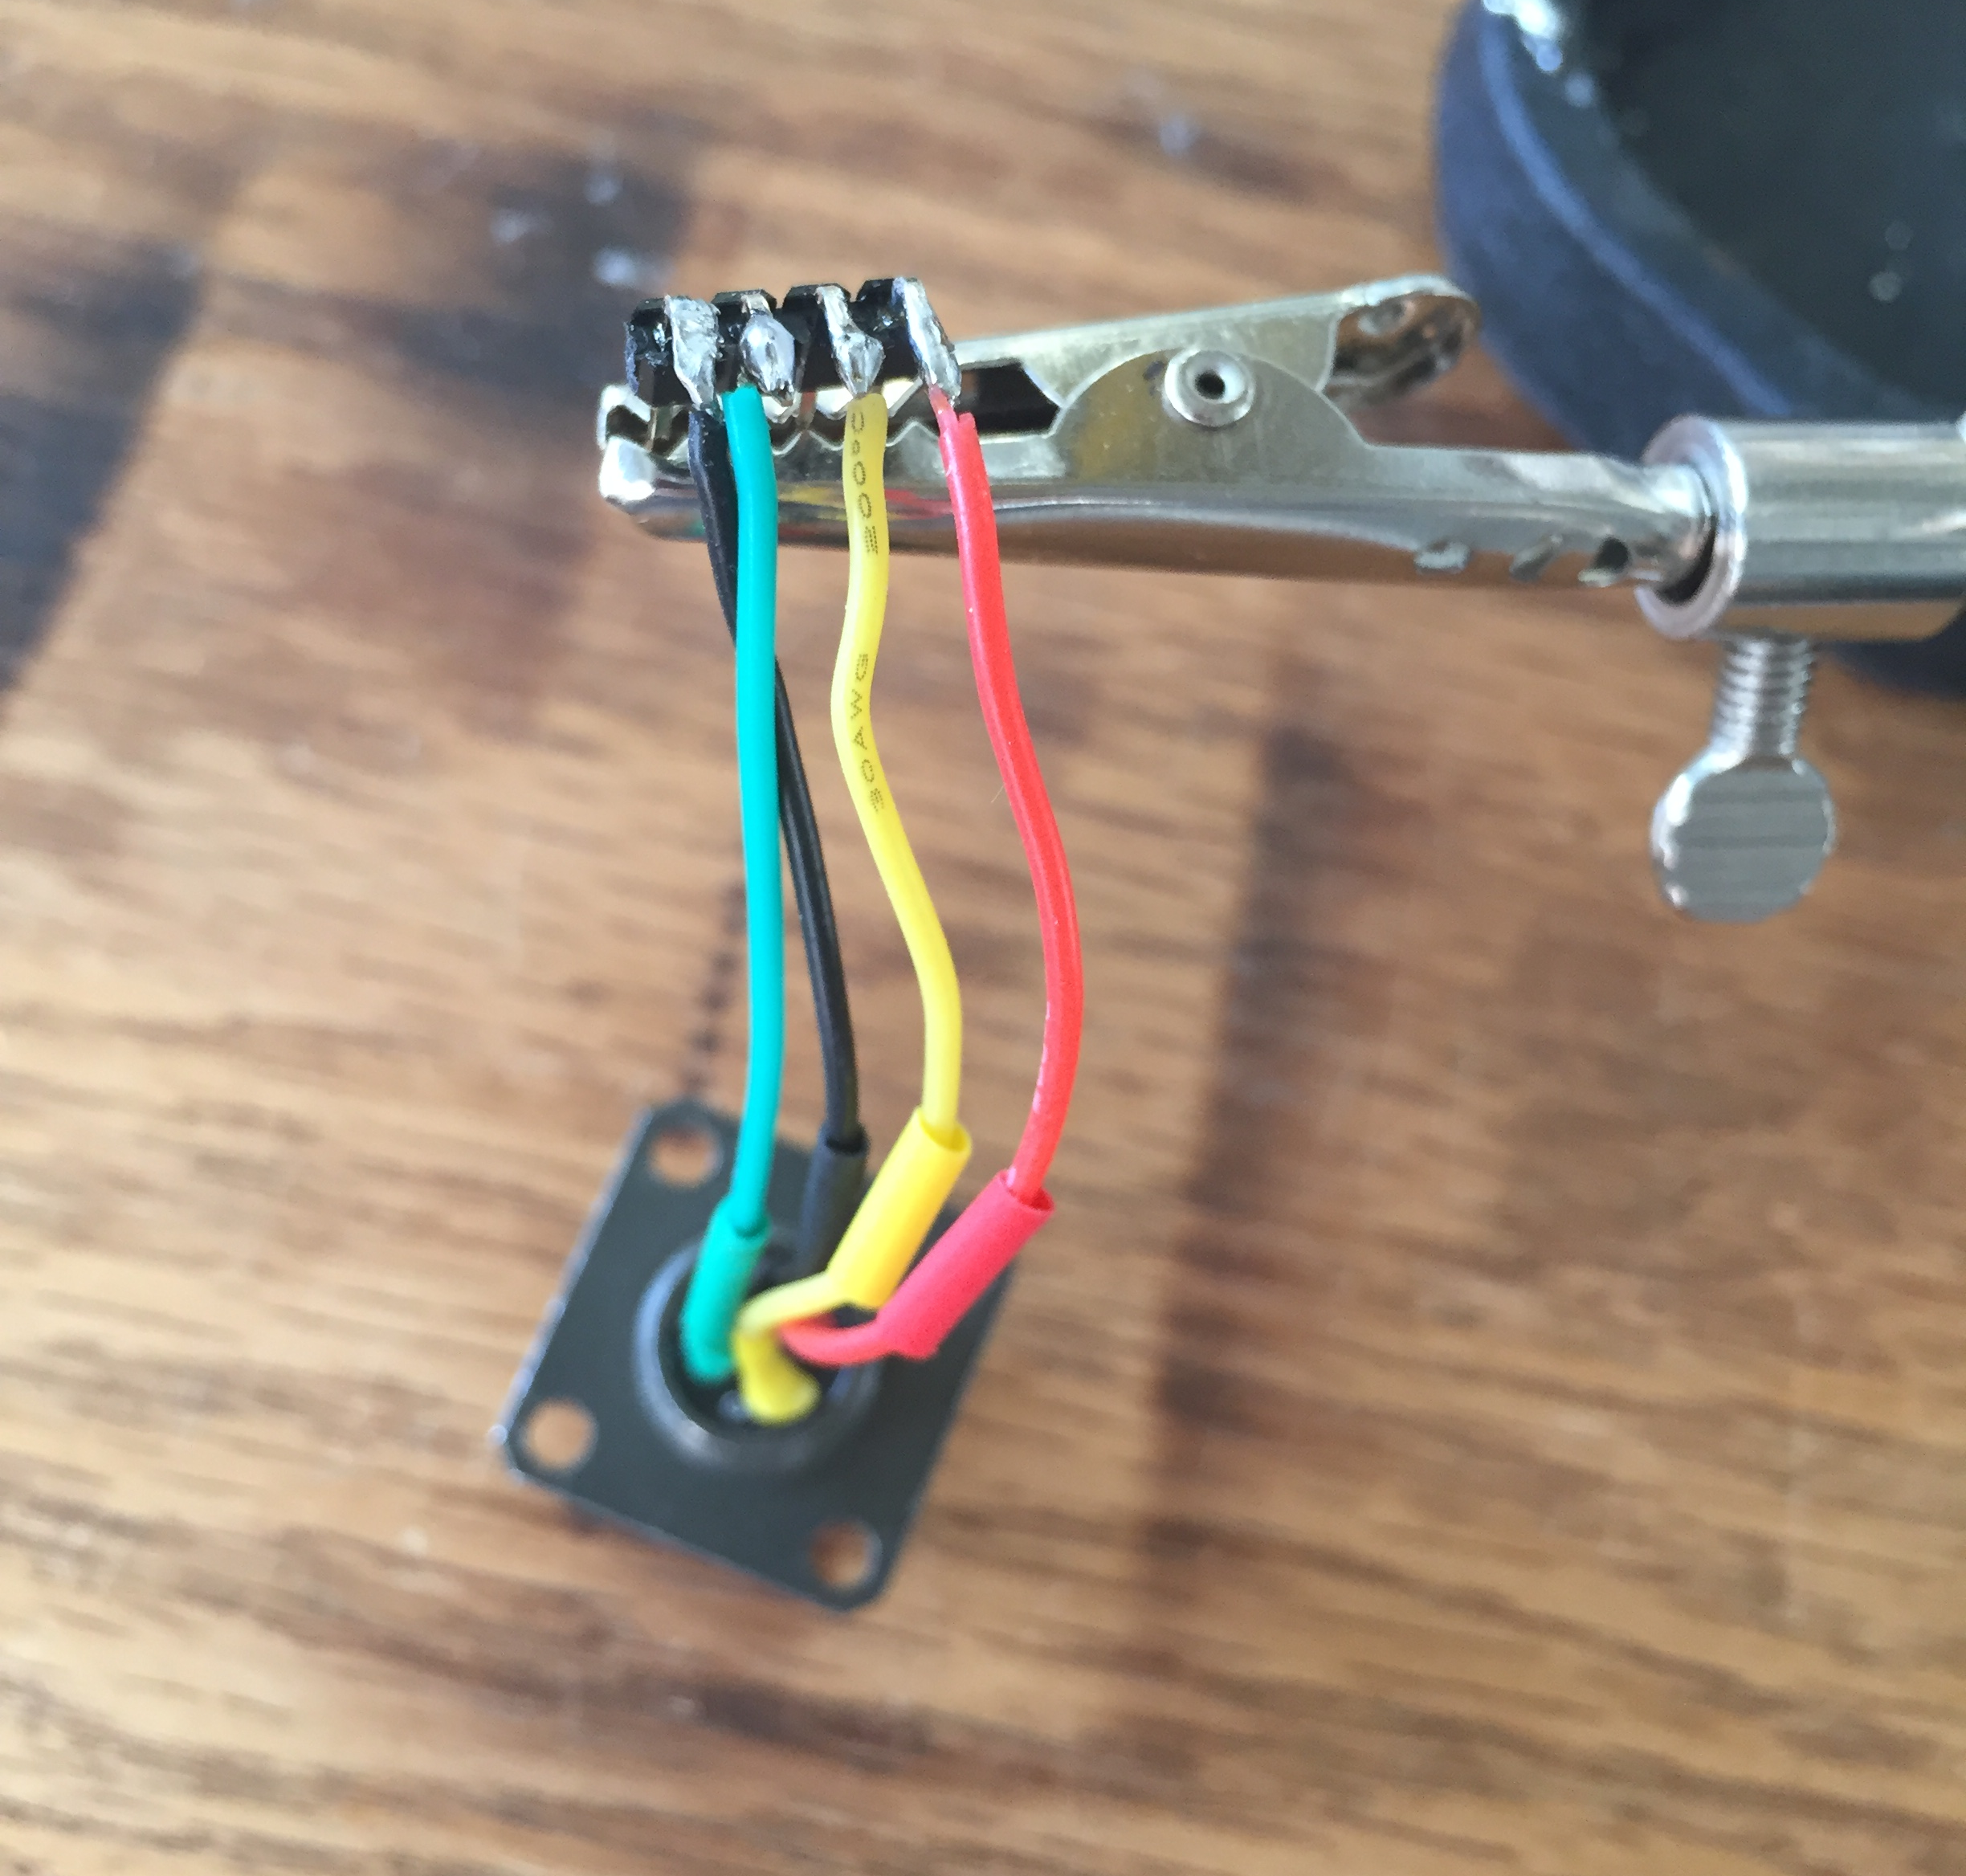
\includegraphics[width=0.6\textwidth]{solder_2.png}
				\caption{Soldering method for connecting 4-pin connector and header pins.}
				\label{fig:solder}
			\end{figure}
			\item While holding the header pins in the helping hands, solder each wire to its corresponding pin, as shown in section \ref{diagram}. It is helpful to wrap the wire around the pin before soldering. Refer to figure~\ref{fig:solder} for soldering setup.
			\item Using the lighter, heat the shrink tube on the 4-pin connector side. Be careful here not to heat the shrink tube on the header side.
		\end{itemize}
	\end{enumerate}


\subsection{Partial Assembly}
	\begin{figure} [h]
		\centering
		\includegraphics[width=0.6\textwidth]{g10_1.png}
		\caption{Orientation of G-10 base for mounting fan on the left and CO$_2$ sensor on the right.}
		\label{fig:g10-fan}
	\end{figure}
	\begin{enumerate}
		\item Mount fan: \\
		\textnormal{With the G-10 oriented as shown in figure~\ref{fig:g10-fan}, put a 2-56 machine screw up through each of the 3 small holes on the left of the G-10 base. Attach each screw to the base with one 2-56 nut. Put a second nut on each screw and position each one to a height of 1/4" above the G-10 base. Set the fan (label side up, wires coming out of lower right corner) onto the three screws. Tighten a third nut onto each screw to hold the fan in place. Using two pliers, tighten the nuts onto the fan to ensure they stay in place.}
		\item Insert: \\
		\textnormal{First, put 4-pin gasket over the header pins and lay it in place on 4-pin connector. Feed the header pins into the aluminum enclosure through the largest hole. Partially screw in the 4-pin connector with four 4-40 screws. The red wire should be in the top right position when the 4-pin connector is fixed in place. Fit the G-10 base with the fan mounted on it into the enclosure.}
		\item Solder fan wires: \\
		\textnormal{Cut the two fan wires to 2" and strip 1/8" of insulation from the wires. Slide the red and black wires through the back of the red and black shrink tube. Solder the red wire to the header with the other red wire. Solder the black wire to the header with the other black wire. Use the lighter to heat the remaining shrink tube as close to the header pins as possible. If the pins or wires are still exposed, apply a small amount of hot glue to them to prevent shorting the pins.}
		\item Attach 4-pin connector: \\
		\textnormal{Remove each screw (one at a time) holding the 4-pin connector in place and apply a small amount of RTV to the screw's threads before screwing it back in place. Wipe any excess RTV from the screw heads with a paper towel (figure~\ref{fig:screwed}). Note that this can all be completed without the CO$_2$ sensor. This partial assembly is shown in figure~\ref{fig:partial_assembly}.}
		\begin{figure} [h]
			\centering
			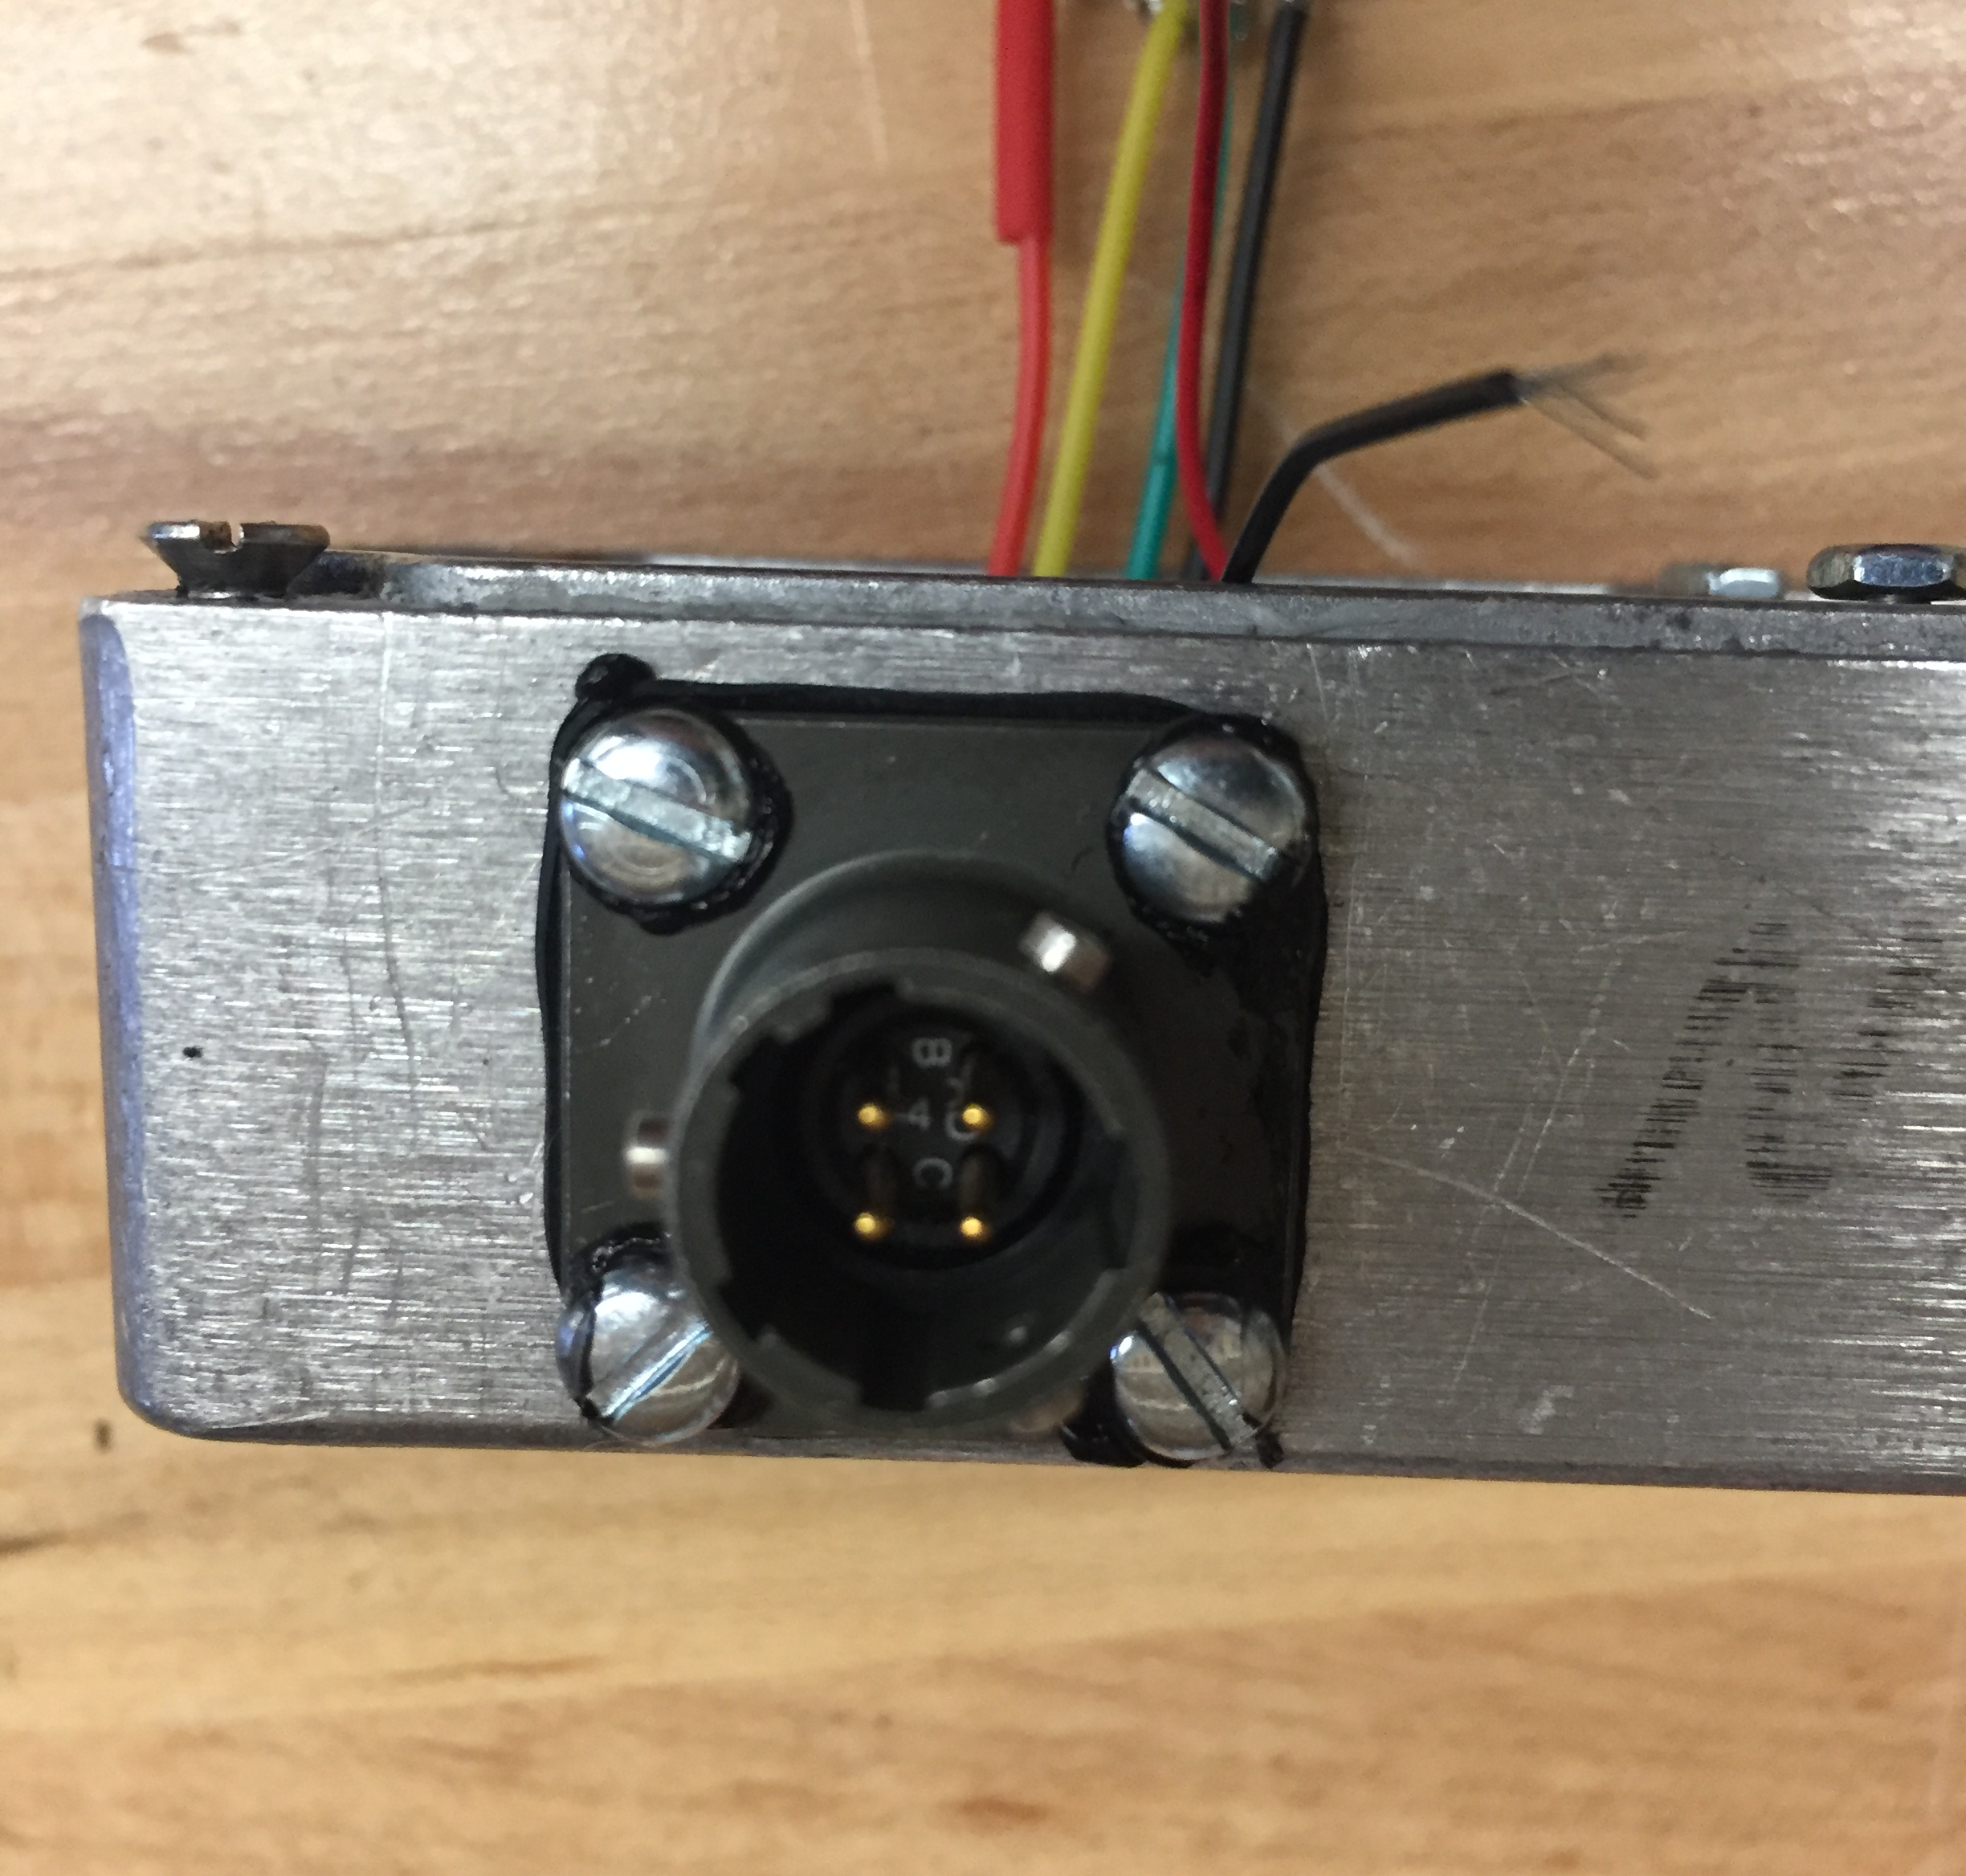
\includegraphics[width=0.6\textwidth]{4pin_screwed_1.png}
			\caption{RTV is applied to the screws. Be sure to clean any excess off to make the boxes uniform in appearance.}
			\label{fig:screwed}
		\end{figure}
		\begin{figure} [h]
			\centering
			\includegraphics[width=0.6\textwidth]{partial_assembly_1.png}
			\caption{Completed partial assembly of  CO$_2$ box.}
			\label{fig:partial_assembly}
		\end{figure}
	\end{enumerate}
	
\subsection{Final Assembly (CO$_2$ Sensor)}
	\begin{enumerate}
		\item Mount CO$_2$ sensor: \\
		\textnormal{Carefully place the CO$_2$ sensor onto the G-10 base such that the side of the sensor with the two female header sets should be oriented towards the 4-pin connector. Once in place, use the dowel end of a cotton swab to apply a bead of hot glue to tack down at least three corners (or sides) of the sensor to the base (figure~\ref{fig:hotglue}).}
		\begin{figure} [h]
			\centering
			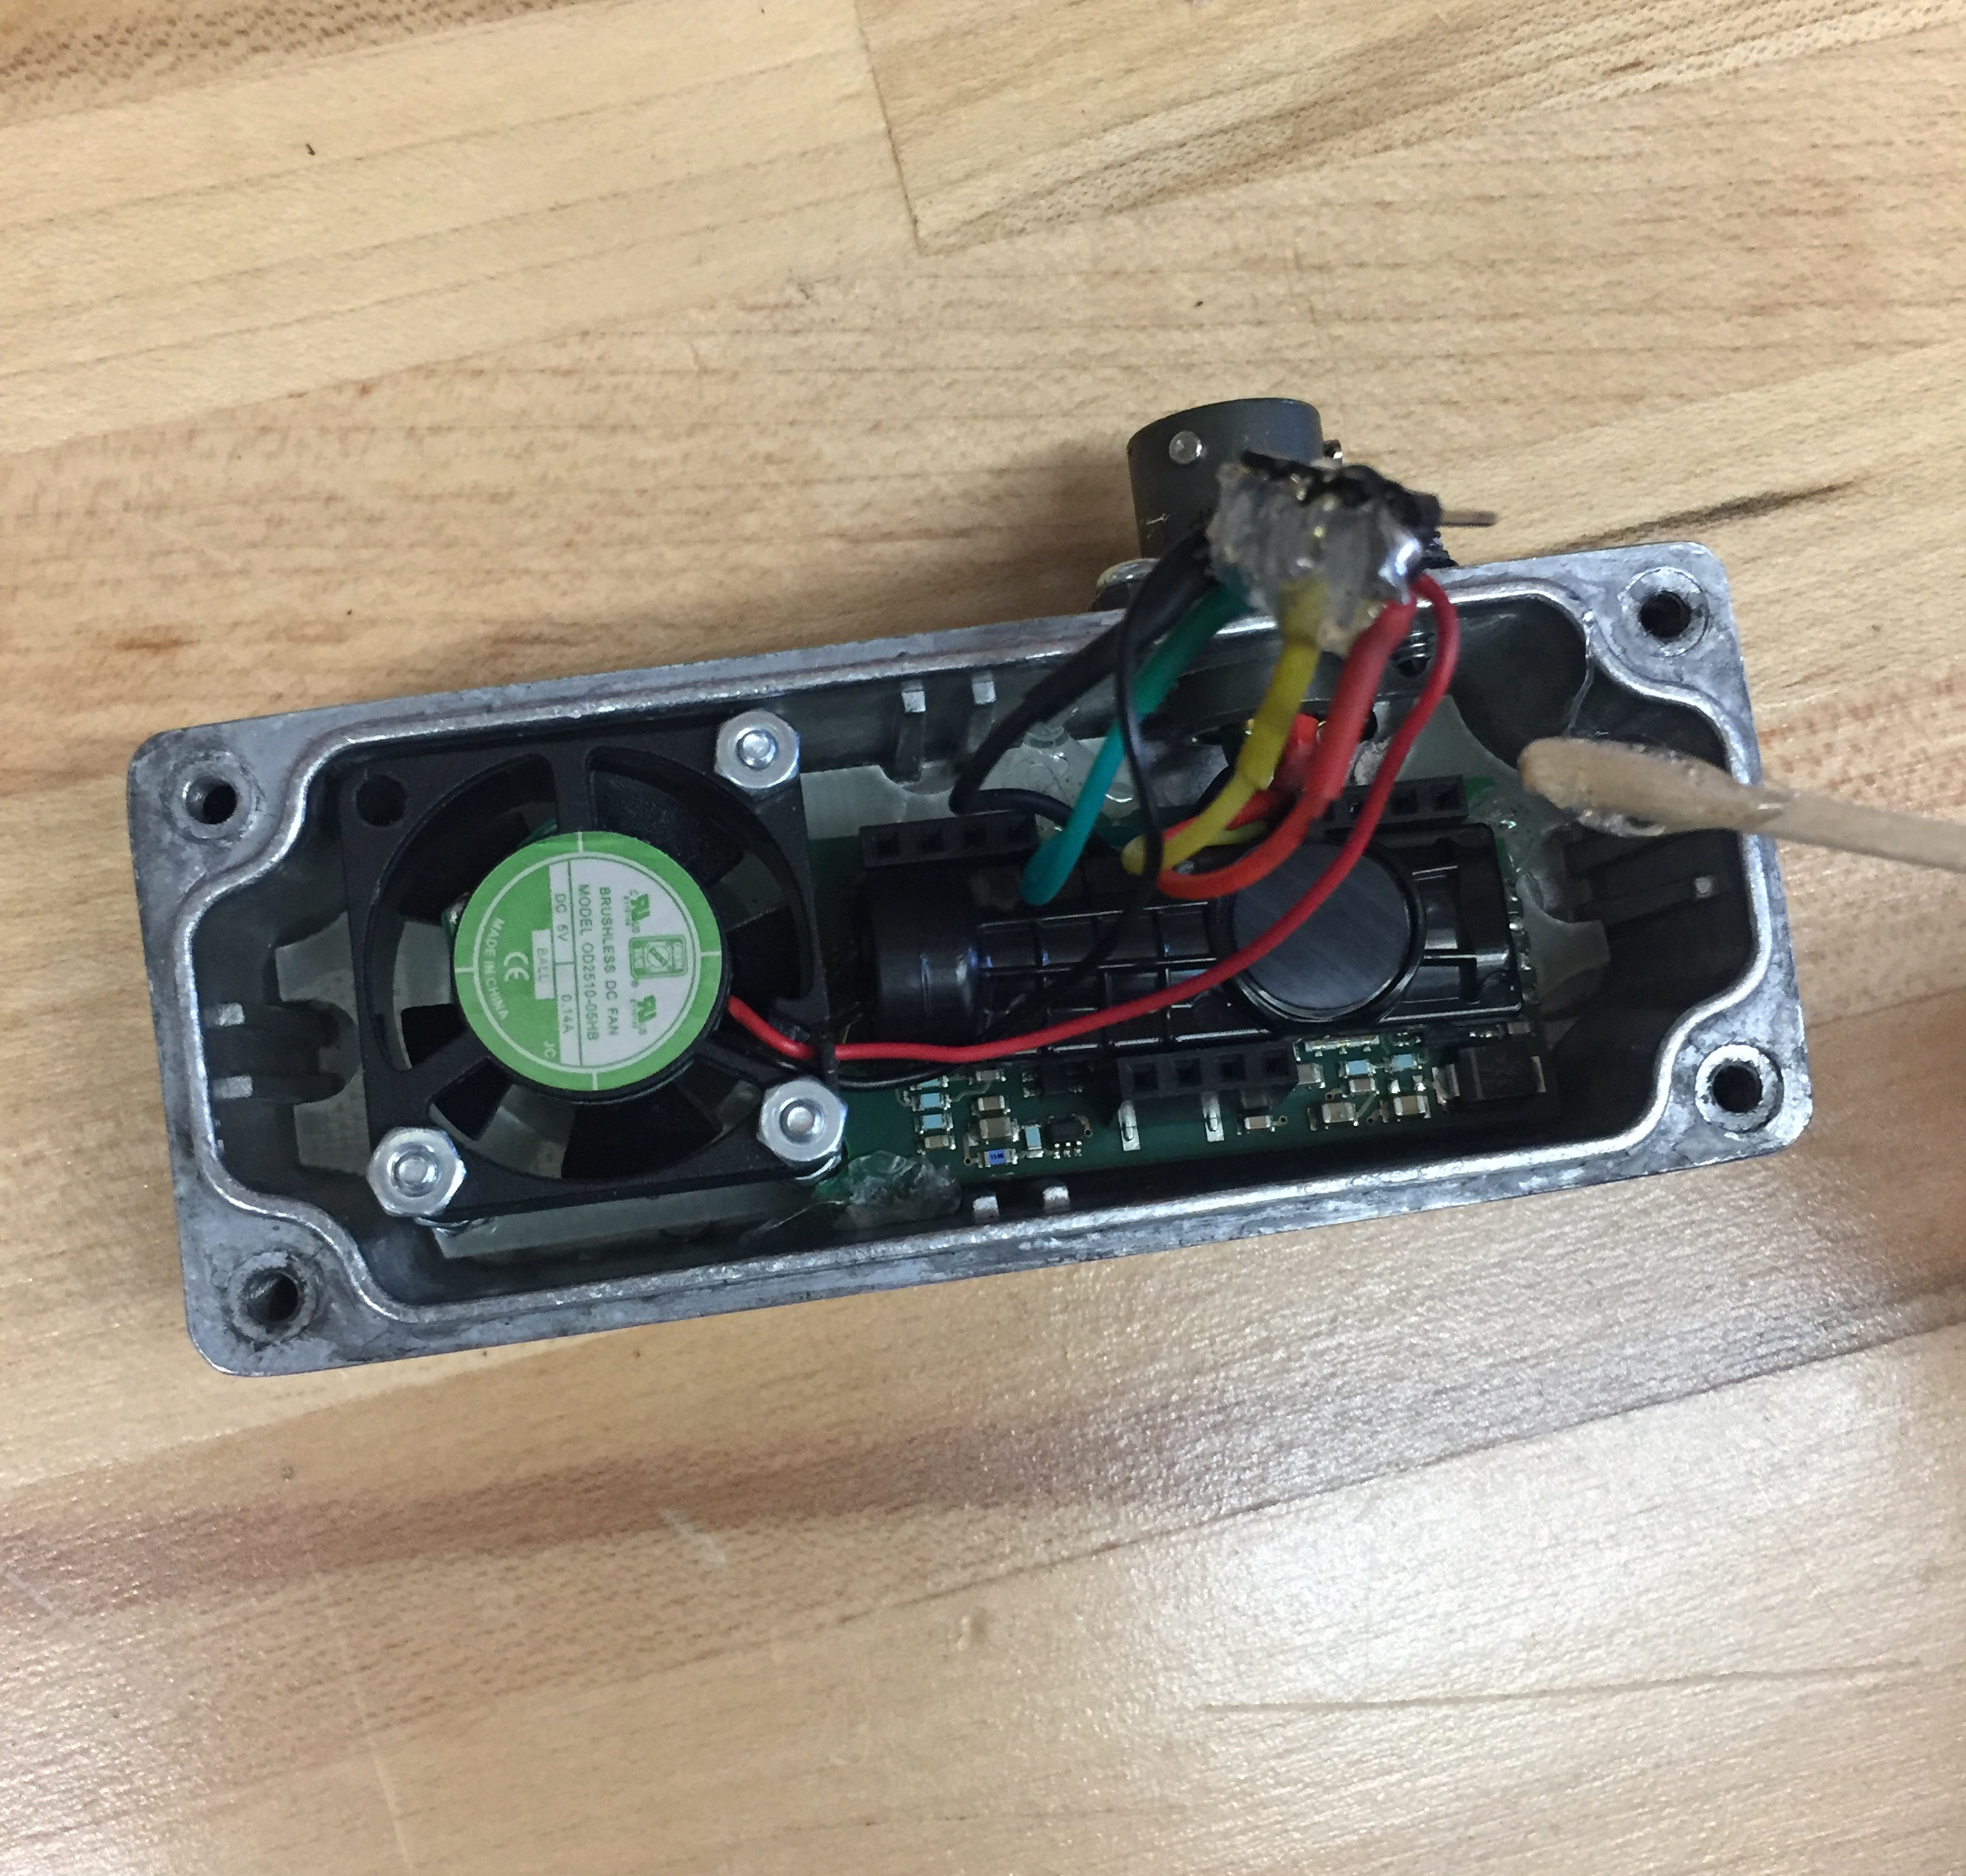
\includegraphics[width=0.6\textwidth]{sensor_hotglue_1.png}
			\caption{Hot gluing CO$_2$ sensor to G-10 base. Here, one bead was added to the bottom, right, and top sides of the sensor.}
			\label{fig:hotglue}
		\end{figure}
		\item Plug in 4-pin connector: \\
		\textnormal{Plug header pins into the top right female header of the CO$_2$ sensor. The completed assembly is shown in figure~\ref{fig:complete}.}
		\begin{figure} [h]
			\centering
			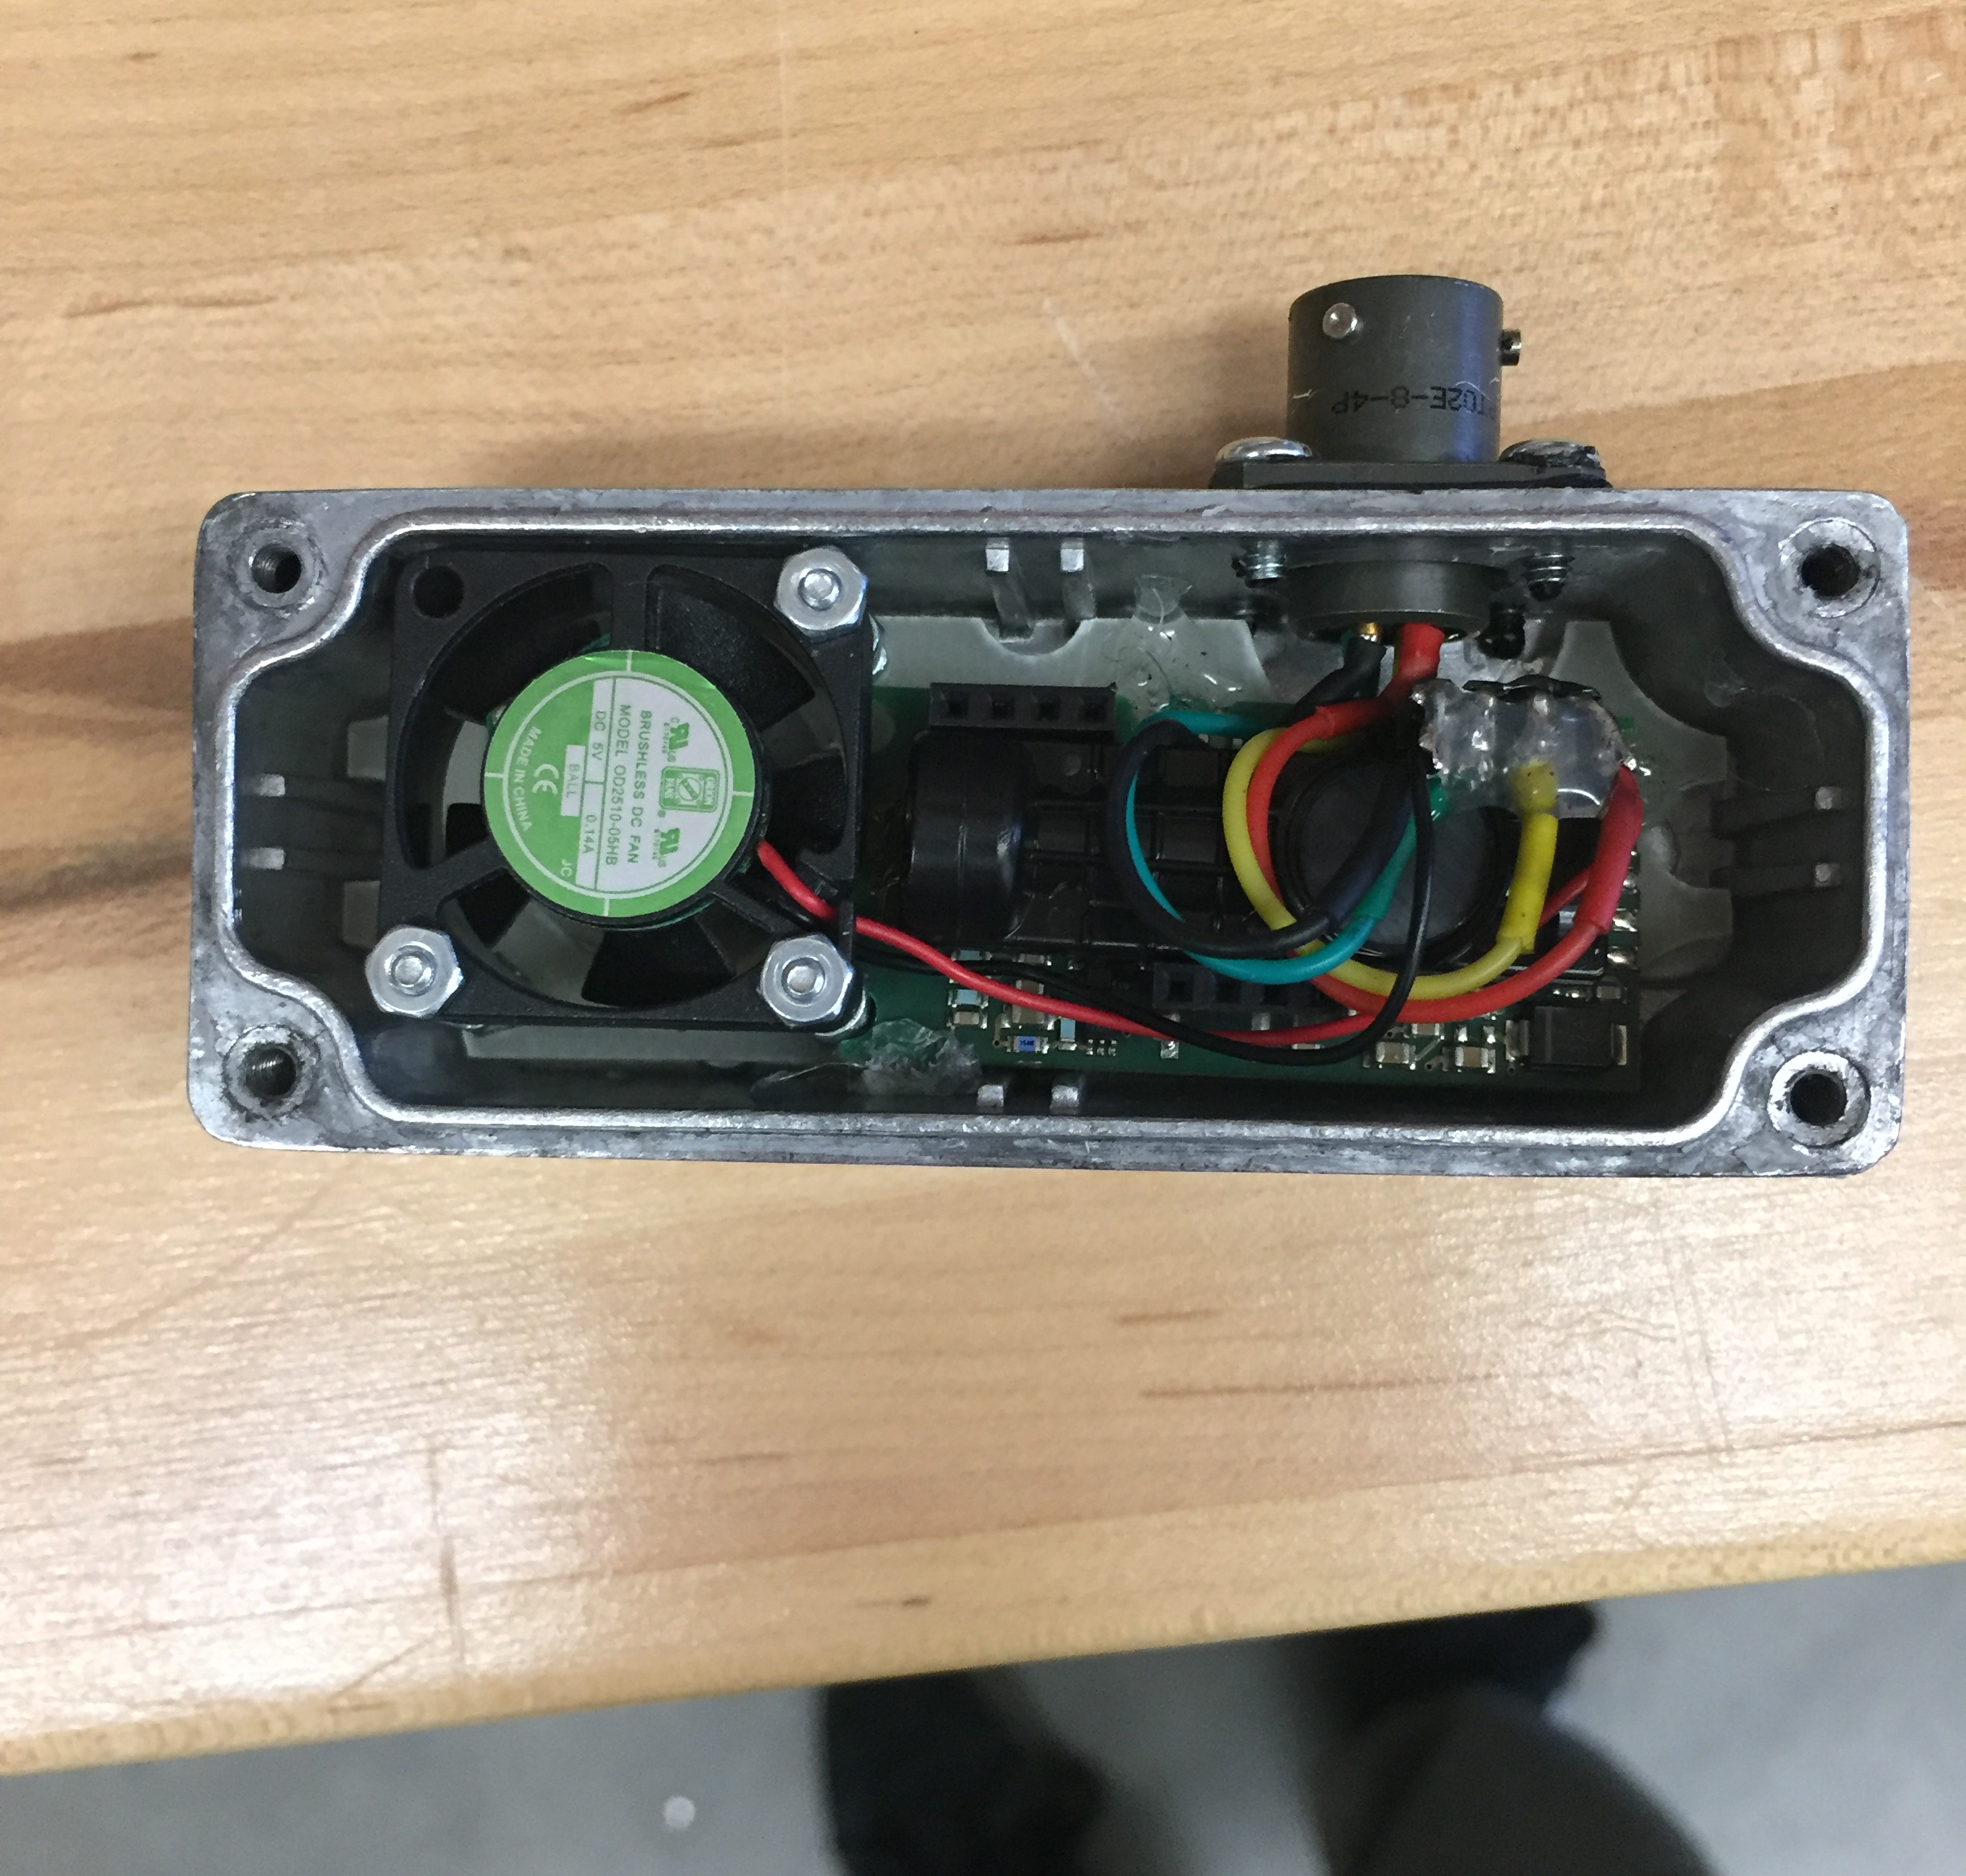
\includegraphics[width=\textwidth]{complete_box_1.png}
			\caption{Completed CO$_2$ box.}
			\label{fig:complete}
		\end{figure}
	\end{enumerate}
	
\subsection{Cleanup}
	\textnormal{Turn off and unplug the soldering iron when assembly is complete. Dispose any wire insulation into the trash receptacle. Put any tooling and materials back in their proper locations.}

\end{document}